\documentclass[11pt]{article}
\usepackage[scaled=0.92]{helvet}
\usepackage{geometry}
\geometry{letterpaper,tmargin=1in,bmargin=1in,lmargin=1in,rmargin=1in}
\usepackage[parfill]{parskip} % Activate to begin paragraphs with an empty line rather than an indent %\usepackage{graphicx}
\usepackage{amsmath,amssymb, mathrsfs, dsfont, stackrel}
\usepackage{tabularx}
\usepackage[font=footnotesize,labelfont=bf]{caption}
\usepackage{graphicx}
\usepackage{xcolor}
%\usepackage[linkbordercolor ={1 1 1} ]{hyperref}
%\usepackage[sf]{titlesec}
\usepackage{natbib}
\usepackage{../../Tianpei_Report}
%\usepackage{appendix}
%\usepackage{algorithm}
%\usepackage{algorithmic}

%\renewcommand{\algorithmicrequire}{\textbf{Input:}}
%\renewcommand{\algorithmicensure}{\textbf{Output:}}



\begin{document}
\title{Lecture 5: Hamiltonian Monte Carlo}
\author{ Tianpei Xie}
\date{Sep. 28th., 2022 }
\maketitle
\tableofcontents
\newpage
\allowdisplaybreaks
\section{Basics of Calculus of Variations}
\subsection{Fundamental theorems of Calculus of Variations}
\begin{itemize}
\item See proof of following lemma from \citep{gelfand2000calculus}.
\begin{lemma} If $\alpha(x)$ is continuous in $[a, b]$, and if
\begin{align}
\int_{a}^{b} \alpha(x) h(x) dx &= 0 \label{eqn: cal_var_lemma_1}
\end{align}
for every continuous function $h(x) \in \cC[a, b]$ such that $h(a) = h(b) = 0$, then $\alpha(x) = 0$
for all $x$ in $[a, b]$
\end{lemma}

\item \begin{lemma} If $\alpha(x)$ is continuous in $[a, b]$, and if
\begin{align*}
\int_{a}^{b} \alpha(x) \dot{h}(x) dx &= 0 
\end{align*}
for every first-order differentiable function $h(x) \in \cD_{1}[a, b]$ such that $h(a) = h(b) = 0$, then $\alpha(x) = c$ constant
for all $x$ in $[a, b]$
\end{lemma}

\item \begin{lemma} If $\alpha(x)$ is continuous in $[a, b]$, and if
\begin{align*}
\int_{a}^{b} \alpha(x) \ddot{h}(x) dx &= 0 
\end{align*}
for every second-order differentiable function $h(x) \in \cD_{2}[a, b]$ such that $h(a) = h(b) = 0$ and $\dot{h}(a) = \dot{h}(b) = 0$, then $\alpha(x) = c_1\,x + c_0$ linear
for all $x$ in $[a, b]$ and $c_0, c_1$ are some constants.
\end{lemma}

\item \begin{lemma} If $\alpha(x), \beta(x)$ are continuous in $[a, b]$, and if
\begin{align}
\int_{a}^{b} \brac{\alpha(x) h(x) + \beta(x) \dot{h}(x)} dx&= 0 \label{eqn: cal_var_lemma_4}
\end{align}
for every first-order differentiable function $h(x) \in \cD_{1}[a, b]$ such that $h(a) = h(b) = 0$, then $\beta(x)$ is differentiable, $\frac{d}{dx}\beta(x) = \alpha(x)$
for all $x$ in $[a, b]$.
\end{lemma}

\item \begin{definition} \citep{gelfand2000calculus}\\
Let $J[y]$ be a \emph{\textbf{functional}} defined on some \emph{normed linear space}, and let
\begin{align*}
\Delta J[h] &= J[y + h] - J[y]
\end{align*} be its \emph{\textbf{increment}}, corresponding to the increment $h = h(x)$ of the "\emph{independent variable}" $y = y(x)$.  If $y$ is fixed, $\Delta J[h]$ is a functional of $h$, in general a nonlinear functional. Suppose that
\begin{align*}
\Delta J[h] &= \phi[h] + \epsilon\norm{h}{}
\end{align*}
where $\phi[h]$ is a linear functional and $\epsilon\rightarrow 0$ as $\norm{h}{} \rightarrow 0$. Then the functional
$J[h]$ is said to be \emph{\textbf{differentiable}}, and the \emph{principal linear part} of the increment $\Delta J[h]$, i.e., the linear functional $\phi[h]$ which differs from $\Delta J[h]$ by an infinitesimal of order higher than $1$ relative to $\norm{h}{} \rightarrow 0$, is called the \underline{\emph{\textbf{variation (or differential)}}} of $J[y]$ and is denoted by $\delta J[h]$.
\end{definition}

\item \begin{theorem} \textbf{(Necessary condition for extreme point of differentiable functional)}  \citep{gelfand2000calculus}\\
A \textbf{necessary condition} for the differentiable functional $J[y]$ to have an extremum for $y = \hat{y}$ is that \textbf{its variation vanish} for $y = \hat{y}$,
i.e., that
\begin{align}
\delta J[h] &= 0 \label{eqn: cal_var_necessary_cond_extreme}
\end{align} for $y = \hat{y}$ and all admissible $h$.
\end{theorem}
\end{itemize}

\subsection{Euler-Lagrange equation}
In the \emph{\textbf{calculus of variations}} \citep{gelfand2000calculus} and \emph{classical mechanics}, the \emph{\textbf{Euler-Lagrange equations}} are a system of second-order ordinary differential equations whose solutions are stationary points of the given action functional. 

\begin{itemize}
\item \textbf{Problem formulation}: Let $F(x, y, z)$ be a function with continuous first and second (partial) derivatives with respect to all its arguments. Then, among
all functions $y(x)$ which are continuously differentiable for $x\in [a, b]$ and
satisfy the boundary conditions
\begin{align*}
y(a) = A, \;y(b) = B,
\end{align*} find the function for which the functional 
\begin{align}
J[y] &= \int_{a}^{b} F(x,\, y,\, \dot{y}) dx  \label{eqn: euler_lagrangian_problem}
\end{align} has a \textbf{\emph{weak extremum}}.

\item \begin{theorem} \textbf{(Euler-Lagrange equations)}  \citep{gelfand2000calculus}\\
Let $J[y]$ be a functional of the forms:
\begin{align}
J[y] &= \int_{a}^{b} F(x,\, y,\, \dot{y}) dx  \label{eqn: euler_lagrangian_problem2}
\end{align} defined on the set of functions $y(x)$ which have continuous first derivatives in $[a, b]$ and satisfy the boundary conditions $y(a) = A, y(b) = B$. Then
a \textbf{necessary condition} for $J[y]$ to have an extremum for a given function $y(x)$ is that $y(x)$ satisfy \textbf{Euler's equation}
\begin{align}
\partdiff{F}{y} - \frac{d}{dx}\partdiff{F}{\dot{y}} &= 0. \label{eqn: euler_lagrange}
\end{align}
\end{theorem}
\begin{proof}
Suppose we give $y(x)$ an increment $h(x)$, where, in order for the function
$y(x) + h(x)$
to continue to satisfy the boundary conditions, we must have $h(a) = h(b) = 0$.

Then, since the corresponding increment of the functional  $\Delta J$ equals
\begin{align*}
\Delta J &= J[y + h] - J[y] = \int_{a}^{b} F(x,\, y+h,\, \dot{y}+\dot{h}) dx - \int_{a}^{b} F(x,\, y,\, \dot{y}) dx\\
&= \int_{a}^{b} \brac{F(x,\, y+h,\, \dot{y}+\dot{h}) - F(x,\, y,\, \dot{y}) }dx,
\end{align*}
it follows by using Taylor's theorem that
\begin{align*}
\Delta J &=  \int_{a}^{b} \brac{\partdiff{F}{y}(x, y, \dot{y})\,h + \partdiff{F}{\dot{y}}(x, y, \dot{y})\,\dot{h}} dx + \ldots,
\end{align*} where  the dots denote terms of order higher than $1$ relative to $h$ and $\dot{h}$. The integral in the right-hand side represents the principal
linear part of the increment $\Delta J[h]$, and hence the variation of $J[y]$ is
\begin{align*}
\delta J  &=  \int_{a}^{b} \brac{\partdiff{F}{y}\,h + \partdiff{F}{\dot{y}}\,\dot{h}} dx.
\end{align*}

Using the necessary condition for extreme $y=y(x)$ of continous functional, we have
\begin{align*}
\delta J[h]   &=  \int_{a}^{b} \brac{\partdiff{F}{y}\,h + \partdiff{F}{\dot{y}}\,\dot{h}} dx =  0
\end{align*} for all admissible $h$. According to Lemma \eqref{eqn: cal_var_lemma_4}, $\alpha(x) = \partdiff{F}{y}$ and $\beta(x) = \partdiff{F}{\dot{y}}$,
\begin{align*}
\partdiff{F}{y} - \frac{d}{dx}\partdiff{F}{\dot{y}} &= 0. \qed
\end{align*}
\end{proof}

\item From geometry point of view, the equation \eqref{eqn: euler_lagrange} is a system of differential equations for the \underline{\textbf{\emph{geodesic}}} between $y(a)$ and $y(b)$.

\item The equation \eqref{eqn: euler_lagrange} can be generalized to multiple variables. Let 
\begin{align}
J[\mb{x}]=  J[x^1, \ldots, x^n] := \int_{a}^{b}\cL(\mb{x}, \dot{\mb{x}}, t)dt =  \int_{a}^{b}\cL(x^1, \ldots, x^n, \dot{x}^1, \ldots, \dot{x}^{n}, t) dt \label{eqn: functional_lagrangian}
\end{align}  be the functional of Lagrangian function.  
The \emph{\textbf{geodesic}} between $\mb{x}(a)$ and $\mb{x}(b)$ is computed by minimizing the functional in \eqref{eqn: functional_lagrangian}. From physics point of view, the integral evaluated along the extremal passing through two given points, i.e., two configurations of the system, is the "least action" corresponding to the motion of the system from the first configuration to the second.

Its solution is given by the \emph{\textbf{Euler-Lagrange equation}}
\begin{align}
\partdiff{\cL}{x^{i}} - \frac{d}{dt}\partdiff{\cL}{\dot{x}^{i}} &= 0, \forall\,i. \label{eqn: euler_lagrange_2}
\end{align}
\end{itemize}




\subsection{Hamilton's equations}
\begin{itemize}
\item 
\begin{definition}
The \emph{\textbf{Hamiltonian (function)}} corresponding to the functional $J[\mb{x}]$ in \eqref{eqn: functional_lagrangian} is defined as 
\begin{align}
\cH( \mb{x}, \mb{v}, t) &:= \inn{\mb{v}}{\dot{\mb{x}}} - \cL(\mb{x}, \dot{\mb{x}}, t) \nonumber\\
\cH(x^1, \ldots, x^n, v_{1}, \ldots,  v_{n}, t) &= \sum_{i}v_i \dot{x}^{i} -  \cL(x^1, \ldots, x^n, \dot{x}^{1}, \ldots,  \dot{x}^{n}, t) \label{eqn: Hamiltonian}
\end{align}
\end{definition}

\item  In this way, we can make a local transformation from the "variables"  $(t, x^1, \ldots, x^n, \dot{x}^{1}, \ldots,  \dot{x}^{n}, \cL)$ appearing in \eqref{eqn: functional_lagrangian} to the new quantities  $(t, x^1, \ldots, x^n, v_{1}, \ldots,  v_{n}, \cH)$, called the \emph{\textbf{canonical variables}} corresponding to the functional $J[\mb{x}] = J[x^1, \ldots, x^n]$.

\item \begin{theorem} \textbf{(Hamilton's equations or The canonical system of Euler's equations )}  \citep{gelfand2000calculus}\\
Let $J[y]$ be a functional of the forms:
\begin{align}
J[x^1, \ldots, x^n] &=\int_{a}^{b}\cL(x^1, \ldots, x^n, \dot{x}^1, \ldots, \dot{x}^{n}, t) dt  \label{eqn: lagrangian_functional}
\end{align} defined on the set of functions $x^{i}(t), i=1,\ldots, n$ which have continuous first derivatives in $[a, b]$ and satisfy the boundary conditions $\mb{x}(a) = [x^{1}(a), \ldots, x^{n}(a)] = A$, $\mb{x}(b) = [x^{1}(b), \ldots, x^{n}(b)] = B$. The Hamiltonian $\cH$ corresponding to functional $J$ is defined as 
\begin{align*}
\cH(x^1, \ldots, x^n, v_{1}, \ldots,  v_{n}, t) &= \sum_{i}v_i \dot{x}^{i} -  \cL(x^1, \ldots, x^n, \dot{x}^{1}, \ldots,  \dot{x}^{n}, t) .
\end{align*}
Then a \textbf{necessary condition} for $J[x^1, \ldots, x^n]$ to have an extremum for a given function $\mb{x}(t) = [x^{1}(t), \ldots, x^{n}(t)]$ is that $\mb{x}(t)$ and $\mb{v}(t)$ satisfy  \underline{\textbf{Hamilton's equations}}
\begin{align}
\partdiff{\cH}{v_{i}} &=  \dot{x}^{i}, \quad \forall\,i \label{eqn: Hamilton_equation_1}\\
\partdiff{\cH}{x^{i}} &= - \partdiff{\cL}{x^{i}} = - \dot{v}_{i}, \quad \forall\,i \label{eqn: Hamilton_equation_2}\\
\partdiff{\cH}{t} &=  - \partdiff{\cL}{t} \label{eqn: Hamilton_equation_3}
\end{align} 
\end{theorem}
\begin{proof} We can find the total differential of Lagrangian function
\begin{align*}
d\cL &= \sum_{i}\partdiff{\cL}{x^{i}}dx^{i} +  \sum_{i}\partdiff{\cL}{\dot{x}^{i}}d\dot{x}^{i} + \partdiff{\cL}{t}dt \\
&=  \sum_{i}\partdiff{\cL}{x^{i}}dx^{i} +  \sum_{i}\brac{d\paren{\partdiff{\cL}{\dot{x}^{i}}\dot{x}^{i}} - \dot{x}^{i}d\paren{\partdiff{\cL}{\dot{x}^{i}}} } + \partdiff{\cL}{t}dt \\
0&=\sum_{i}d\paren{\partdiff{\cL}{\dot{x}^{i}}\dot{x}^{i}} - d\cL +  \sum_{i}\partdiff{\cL}{x^{i}}dx^{i} -  \sum_{i} \dot{x}^{i}d\paren{\partdiff{\cL}{\dot{x}^{i}}} + \partdiff{\cL}{t}dt \\
&= \sum_{i}d\paren{\partdiff{\cL}{\dot{x}^{i}}\dot{x}^{i}-\cL}  +  \sum_{i}\brac{\partdiff{\cL}{x^{i}}dx^{i} -  \dot{x}^{i}d\paren{\partdiff{\cL}{\dot{x}^{i}}}} + \partdiff{\cL}{t}dt \\
d\paren{\sum_{i}\partdiff{\cL}{\dot{x}^{i}}\dot{x}^{i}-\cL} &=   \sum_{i}\brac{-\partdiff{\cL}{x^{i}}dx^{i} +  \dot{x}^{i}d\paren{\partdiff{\cL}{\dot{x}^{i}}}} - \partdiff{\cL}{t}dt  \\
d\paren{\sum_{i}v_i\dot{x}^{i}-\cL} &=   \sum_{i}\paren{-\partdiff{\cL}{x^{i}}}dx^{i} + \sum_{i} \dot{x}^{i}dv_i - \partdiff{\cL}{t}dt \quad \text{ let }v_i := \partdiff{\cL}{\dot{x}^{i}} \\
d\cH &= \sum_{i}\paren{-\partdiff{\cL}{x^{i}}}dx^{i} + \sum_{i} \dot{x}^{i}dv_i  - \partdiff{\cL}{t}dt \\
\text{Also }d\cH &= \sum_{i}\partdiff{\cH}{x^{i}}dx^{i}  + \sum_{i}\partdiff{\cH}{v_{i}}dv_i + \partdiff{\cH}{t}dt
\end{align*}
Therefore we have 
\begin{align*}
\partdiff{\cH}{x^{i}} &= - \partdiff{\cL}{x^{i}} =  - \frac{d}{dt}\partdiff{\cL}{\dot{x}} = - \dot{v}_{i} \quad \text{(by Euler-Lagrange equation)}\\
\partdiff{\cH}{v_{i}} &=  \dot{x}^{i} \\
\partdiff{\cH}{t} &=  - \partdiff{\cL}{t} \qed
\end{align*} 
\end{proof}
\item In the case of time-independent $\cH$ and $\cL$, i.e. $\partdiff{\cH}{t} =  - \partdiff{\cL}{t} = 0$, the \underline{\emph{\textbf{Hamiltonian dynamic}}} is defined by $2n$ first-order differential equations:
\begin{align}
\frac{d x^{i}}{dt} &=  \partdiff{\cH}{v_{i}}, \quad  i=1,\ldots, n \nonumber\\
\frac{d v_{i}}{dt} &= - \partdiff{\cH}{x^{i}}, \quad  i=1,\ldots, n \label{eqn: Hamilton_dynamics_general}\\
\Rightarrow \frac{d\mb{z}}{dt} &= \mb{\Omega}\,\grad{\mb{z}}{\cH} \label{eqn: Hamilton_dynamics_general_combine}
\end{align} where $\mb{z}:= (\mb{x}, \mb{v})$ and $\mb{\Omega} = \brac{\begin{array}{cc}
\mb{0} & \mb{I}_{n}  \\
-\mb{I}_{n}  & \mb{0}  
\end{array}}$. 
These differential equations describes the dynamic of a particle moving along the \textbf{geodesic curve} from \emph{\textbf{position}} $\mb{x}(a)$ with \emph{\textbf{velocity}} (or \emph{\textbf{momentum}}) $\mb{v}(a)$ (i.e. configuration $(\mb{x}(a), \mb{v}(a))$) to position $\mb{x}(b)$ with $\mb{v}(b)$ (i.e. configuration $(\mb{x}(b), \mb{v}(b))$). The vector $\mb{v}$ defines a \emph{\textbf{vector fields}} that is \emph{tangent} to the \emph{potential} $\cL$ at position $\mb{x}$.

\item An alternative representation for Hamiltonian dynamic is called \emph{\textbf{variational equations}} \citep{leimkuhler2004simulating}:
\begin{align}
\frac{d}{dt}\mb{\xi} &= \mb{\Omega}\, \nabla^{2}_{\mb{z},\mb{z}}\cH(\mb{z}_t)\, \mb{\xi}.\label{eqn: Hamilton_dynamics_general_variational}
\end{align} where $\mb{\xi}(t) = \partial_{\mb{z}}\phi_{t}(\mb{z}_0)\, \delta \mb{z}_0$ for Hamiltonian flow map $\phi_{t}$.


\item The definition of Hamiltonian can be formulated as the sum of \emph{\textbf{kinetic energy}} $\cK$ and \emph{\textbf{potential energy}} $\cV$ (i.e. \emph{frictionless} motion).

\item The Hamiltonian dynamic captures the \textbf{geometry} of surface by specifying the vector field $\mb{F}= (\frac{d \mb{x}}{dt}, \frac{d \mb{v}}{dt})$ on the surface.
\end{itemize}

\subsection{Properties of Hamiltonian dynamics}
Let the \emph{\textbf{Hamiltonian flow}} $\phi_t : (\mb{x}, \mb{v}) \mapsto (\mb{x}_t(\mb{x}, \mb{v}), \mb{v}_t(\mb{x}, \mb{v}))$ be the position and velocity
after time $t$ starting from $(\mb{x}, \mb{v})$.  The Hamiltonian flow satisfies following \emph{\textbf{properties}}:
\begin{enumerate}
\item \underline{\emph{\textbf{Reversibility}}}: Hamiltonian dynamics of the form mentioned above are \emph{\textbf{time reversible}} for $t \ge 0$:
\begin{align}
\phi_t(\mb{x}_t(\mb{x}, \mb{v}), -\mb{v}_t(\mb{x}, \mb{v})) &= (\mb{x}, -\mb{v}). \label{eqn: Hamiltonian_reverse}
\end{align} The mapping $\phi_t : (\mb{x}, \mb{v}) \mapsto (\mb{x}_t(\mb{x}, \mb{v}), \mb{v}_t(\mb{x}, \mb{v}))$ is one-to-one and has inverse mapping.

\item  \underline{\emph{\textbf{Conservation of the Hamiltonian}}}: A second property of the dynamics is that it keeps the \emph{\textbf{Hamiltonian invariant}} (i.e. \emph{conserved}).
\begin{align}
\frac{d\cH}{dt} &= \sum_{i=1}^{n}\brac{\frac{d x^{i}}{dt}\partdiff{\cH}{x^{i}} + \frac{d v_i}{dt}\partdiff{\cH}{v_{i}} } \nonumber\\
&= \sum_{i=1}^{n}\brac{\frac{d x^{i}}{dt} \frac{d v_i}{dt} - \frac{d v_i}{dt}\frac{d x^{i}}{dt} }  = 0   \label{eqn: Hamiltonian_conserve}
\end{align} To see this note that, since $\cH$ does not depend on $t$ explicitly (or $\partdiff{\cH}{t} = 0$).

\item  \underline{\emph{\textbf{Volume Preservation}}}: A third fundamental property of Hamiltonian dynamics is that it \textbf{\emph{preserves volume in phase space}} $(\mb{x}, \mb{v})$ space. Formally, let $\mb{F}= (\frac{d \mb{x}}{dt}, \frac{d \mb{v}}{dt})$ be the vector field associated to the Hamiltonian in the phase space $\bR^n \times \bR^{n}$. First note that the \emph{\textbf{divergence} of $\mb{F}$ is \textbf{zero}}:
\begin{align}
\nabla \cdot \mb{F} = \text{div}\,\mb{F} &= \sum_{i=1}^{n}\brac{\partdiff{}{x^{i}}\frac{d x^{i}}{dt} +  \partdiff{}{v_{i}}\frac{d v_{i}}{dt}} \nonumber\\
&= \sum_{i=1}^{n}\brac{\partdiff{}{x^{i}}\partdiff{\cH}{v_{i}}  -  \partdiff{}{v_{i}}\partdiff{\cH}{x^{i}} } = 0\label{eqn: Hamiltonian_vol_conserve}
\end{align} Since divergence represents the volume density of the outward flux of a vector field from an infinitesimal volume around a given point, it being zero everywhere implies volume preservation. 

Another way to see this is that divergence is the \emph{\textbf{trace}} of the \emph{\textbf{Jacobian}} of the map $\mb{F}$, and the trace of the Jacobian is the \textbf{\emph{derivative}} of the \emph{\textbf{determinant of the Jacobian}}. Hence, the trace being $0$ implies that the determinant of the Jacobian of $\mb{F}$ does not change.

\item \underline{\emph{\textbf{Symplecticness}}}: Volume preservation is also a consequence of Hamiltonian dynamics being \emph{\textbf{symplectic}}. Let $\mb{z} = (\mb{x}, \mb{v})$, and define $\mb{\Omega}$ as 
\begin{align*}
\mb{\Omega} &= \brac{\begin{array}{cc}
\mb{0} & \mb{I}_{n}  \\
-\mb{I}_{n}  & \mb{0}  
\end{array}}.
\end{align*}  Note $\mb{\Omega}^{-1} = \mb{\Omega}^{T} = -\mb{\Omega}$. 

The \emph{\textbf{symplecticness condition}} is that the Jacobian matrix, $\paren{\partial_{\mb{z}}\mb{\phi}_t}$ of the mapping $\phi_t$ satisfies
\begin{align}
\paren{\partial_{\mb{z}}\mb{\phi}_t}^{T}\mb{\Omega}^{-1}\paren{\partial_{\mb{z}}\mb{\phi}_t} &= \mb{\Omega}^{-1} \label{eqn: symplecticness}
\end{align} This implies volume conservation, since $\det\paren{\partial_{\mb{z}}\mb{\phi}_t}^{T}\,\det\paren{\mb{\Omega}^{-1}}\, \det\paren{\partial_{\mb{z}}\mb{\phi}_t} = \det\paren{\mb{\Omega}^{-1}}$ implies that
$\det{\paren{\partial_{\mb{z}}\mb{\phi}_t}}$ is one. When $n > 1$, the \emph{\textbf{symplecticness condition is stronger than volume preservation}}. Hamiltonian dynamics and the symplecticness condition can be generalized to where $\mb{\Omega}$ is any matrix for which $\mb{\Omega}^{T} =  \mb{\Omega}^{-1}$ and $\det{\mb{\Omega}} \neq 0$.
\end{enumerate} 

Crucially, reversibility, preservation of volume, and symplecticness can be maintained exactly even when, as is necessary in practice, Hamiltonian dynamics is approximated.

\newpage
\section{Markov Chain Monte Carlo from Hamiltonian Dynamics}
\subsection{Monte Carlo in high dimensional spaces}
\begin{itemize}
\item One of the characteristic properties of \textbf{high-dimensional spaces} is that there is \emph{much more volume outside any given neighborhood than inside of it}. Figure \ref{fig: concentration_measure_ball} shows that as the dimensionality increases, more vol lies in the shell of the ball not in the core. 

\begin{figure}
\begin{minipage}[t]{1\linewidth}
  \centering
  \centerline{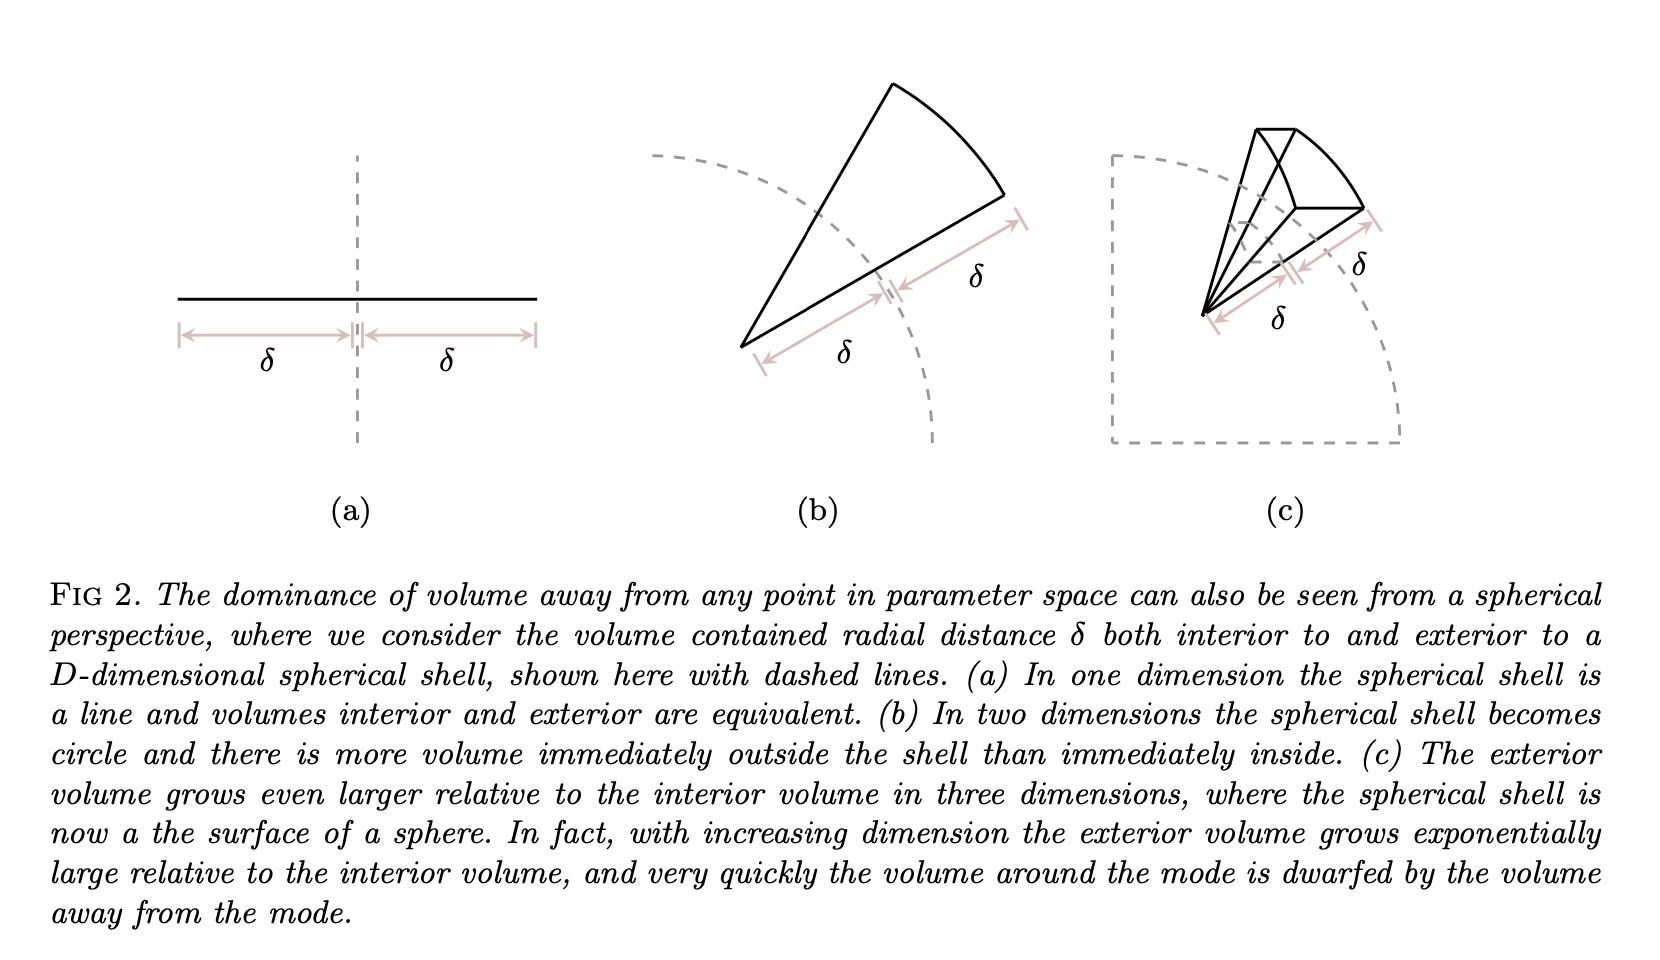
\includegraphics[scale = 0.5]{concentration_measure_ball.png}}
\end{minipage}
\caption{\footnotesize{\textbf{The concentration of measure around the shell of a unit ball \citep{betancourt2017conceptual}}}}
\label{fig: concentration_measure_ball}
\end{figure}

\item On the other hand, the complimentary neighborhood \emph{\textbf{far away from the mode}} features a \emph{much larger volume}, but the \emph{\textbf{vanishing densities}} lead to similarly negligible contributions expectations.  The only significant contributions come from the neighborhood between these two extremes known as \underline{\emph{\textbf{the typical set}}}. (Figure \ref{fig: typical_set}) The Importantly, because probability densities and volumes transform oppositely under any \emph{\textbf{reparameterization}}, the typical set is an invariant object that does not depend on the irrelevant details of any particular choice of parameters. %\emph{Importance Sampling} puts high weights on the typical set to emphasize its contribution. 

\begin{figure}
\begin{minipage}[t]{1\linewidth}
  \centering
  \centerline{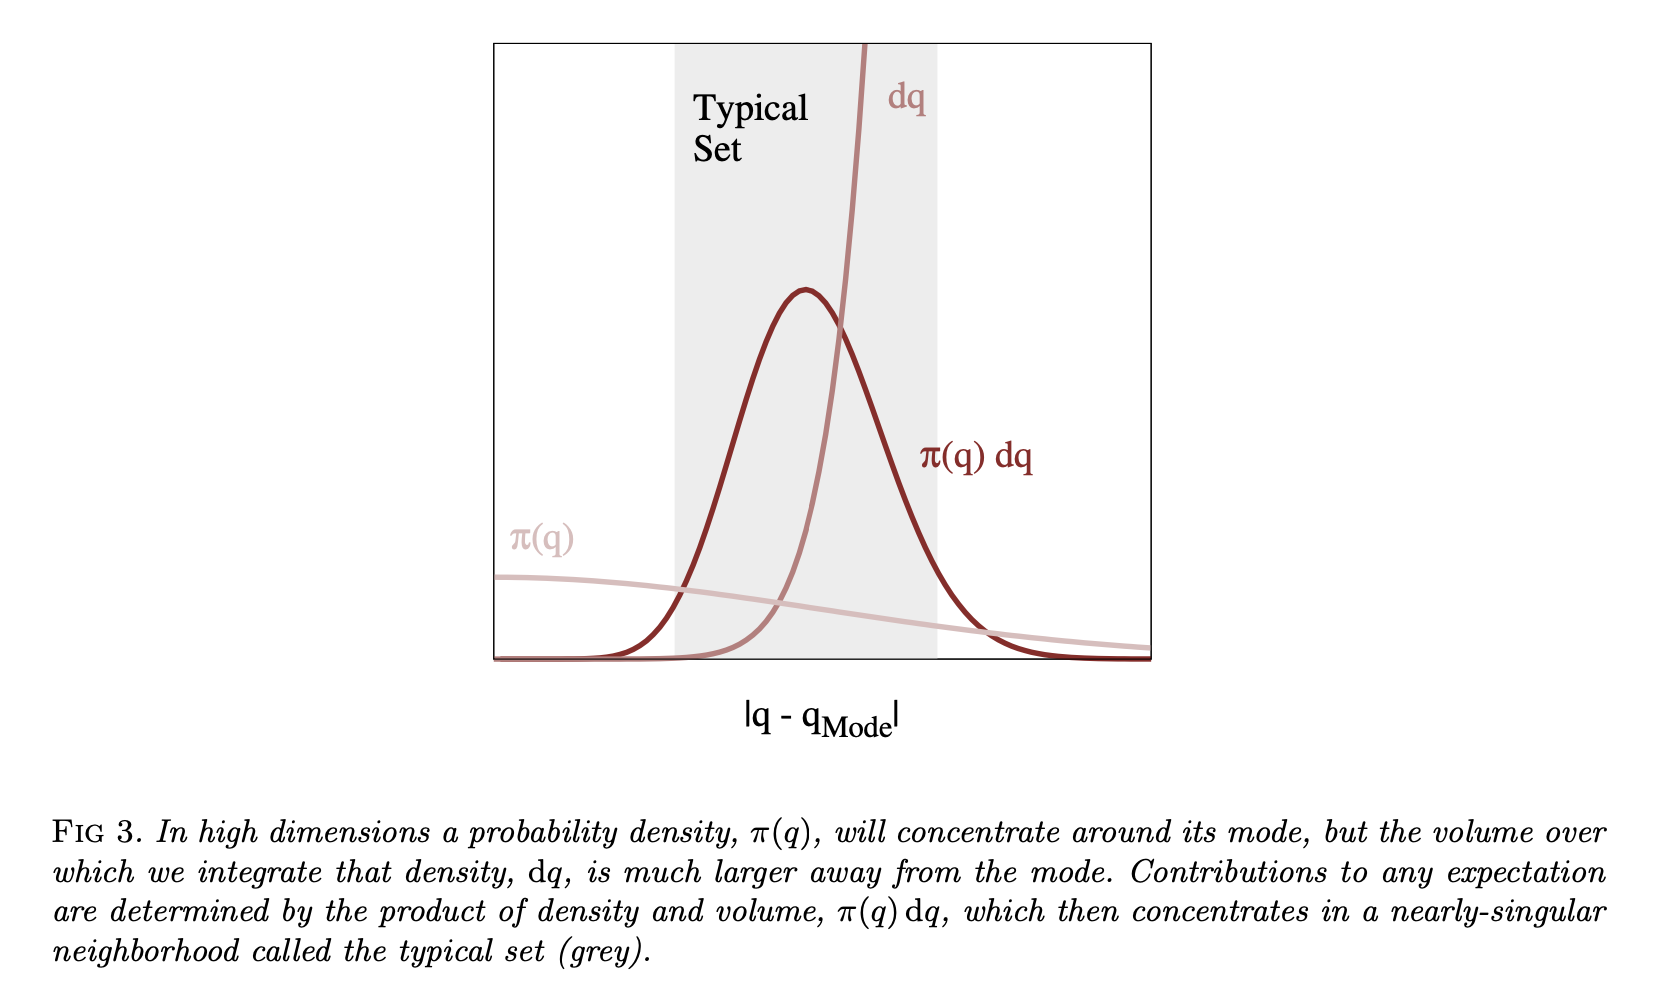
\includegraphics[scale = 0.5]{typical_set.png}}
\end{minipage}
\caption{\footnotesize{\textbf{The typical set of $\pi(q)dq$ is not close to the mode nor far away from it. \citep{betancourt2017conceptual}}}}
\label{fig: typical_set}
\end{figure}

As the dimension of parameter space increases, however,  the tension between the density and the volume grows and the typical set becomes \emph{more singular}.
%As the dimension of parameter space increases, the tension between the density and the volume grows and the regions where the density and volume are both large enough to yield a significant contribution becomes more and more narrow. Consequently the typical set becomes more singular with increasing dimension.

\item The \textbf{success} of Markov Chain Monte Carlo lies in its ability to explore the parameter space while preserving the target distribution. The resulting Markov chain will drift into and then across the typical set regardless of its initial state, providing a powerful quantification of the typical set from which we can derive accurate expectation estimators.

\item Under ideal conditions, Markov chains explore the target distribution in \textbf{three distinct phases} \citep{betancourt2017conceptual}:
\begin{enumerate}
\item In the first phase the Markov chain \emph{converges towards} the typical set from its initial position in parameter space while the Markov chain Monte Carlo estimators suffer from \emph{\textbf{strong biases}}. Consequently, it is common practice to \emph{\textbf{warm up}} the Markov chain by throwing away those initial converging samples before computing Markov chain Monte Carlo estimators \citep{liu2001monte}. 
\item The second phase begins once the Markov chain finds the typical set and persists through the first sojourn across the typical set. This initial exploration is extremely effective and the accuracy of Markov chain Monte Carlo estimators rapidly improves as the bias from the initial samples is eliminated.
\item The third phase consists of all subsequent exploration where the Markov chain refines its exploration of the typical set and the precision of the Markov chain Monte Carlo estimators improves, albeit at a slower rate. In this phase, the central limit theorem holds.
\end{enumerate}

\item Random Walk Metropolis-Hastings is \textbf{doomed to fail} in high dimensional space due to its inefficiency and low acceptance rate. There are an exponential number of directions in which to guess but only a singular number of directions that stay within the typical set and pass the check. (Figure \ref{fig: random_walk_high_dim}) Regardless of how we tune the covariance of the Random Walk Metropolis proposal or the particular details of the target distribution, the resulting Markov chain will explore the typical set extremely slowly in all but the lowest dimensional spaces. 

\begin{figure}
\begin{minipage}[t]{1\linewidth}
  \centering
  \centerline{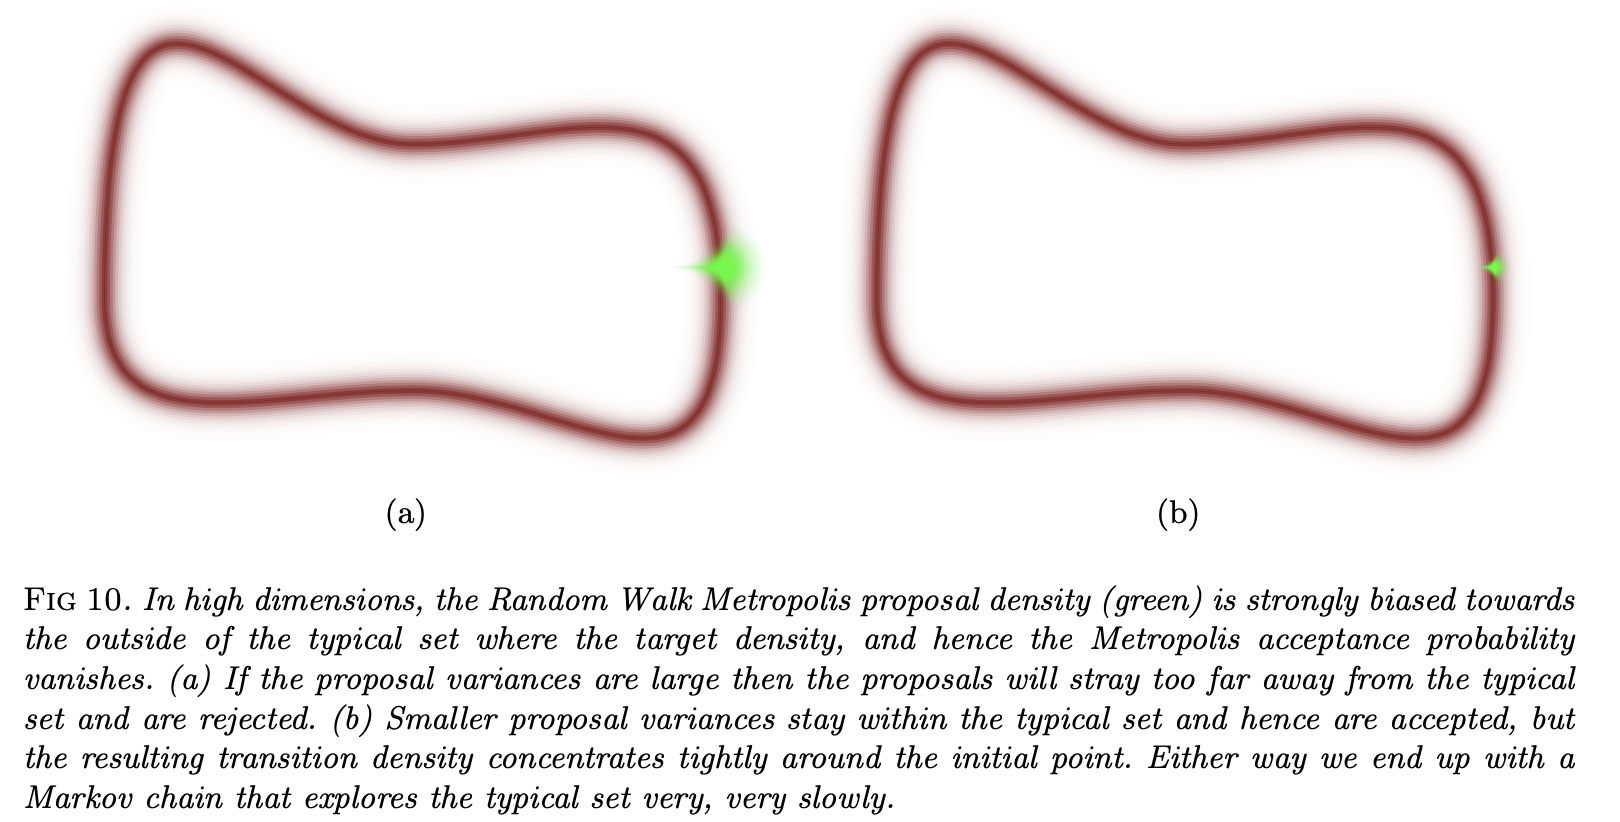
\includegraphics[scale = 0.5]{random_walk_high_dim.png}}
\end{minipage}
\caption{\footnotesize{\textbf{The challenge of random walk Metropolis-Hastings on high dimensional space.  \citep{betancourt2017conceptual}}}}
\label{fig: random_walk_high_dim}
\end{figure}

\begin{figure}
\begin{minipage}[t]{1\linewidth}
  \centering
  \centerline{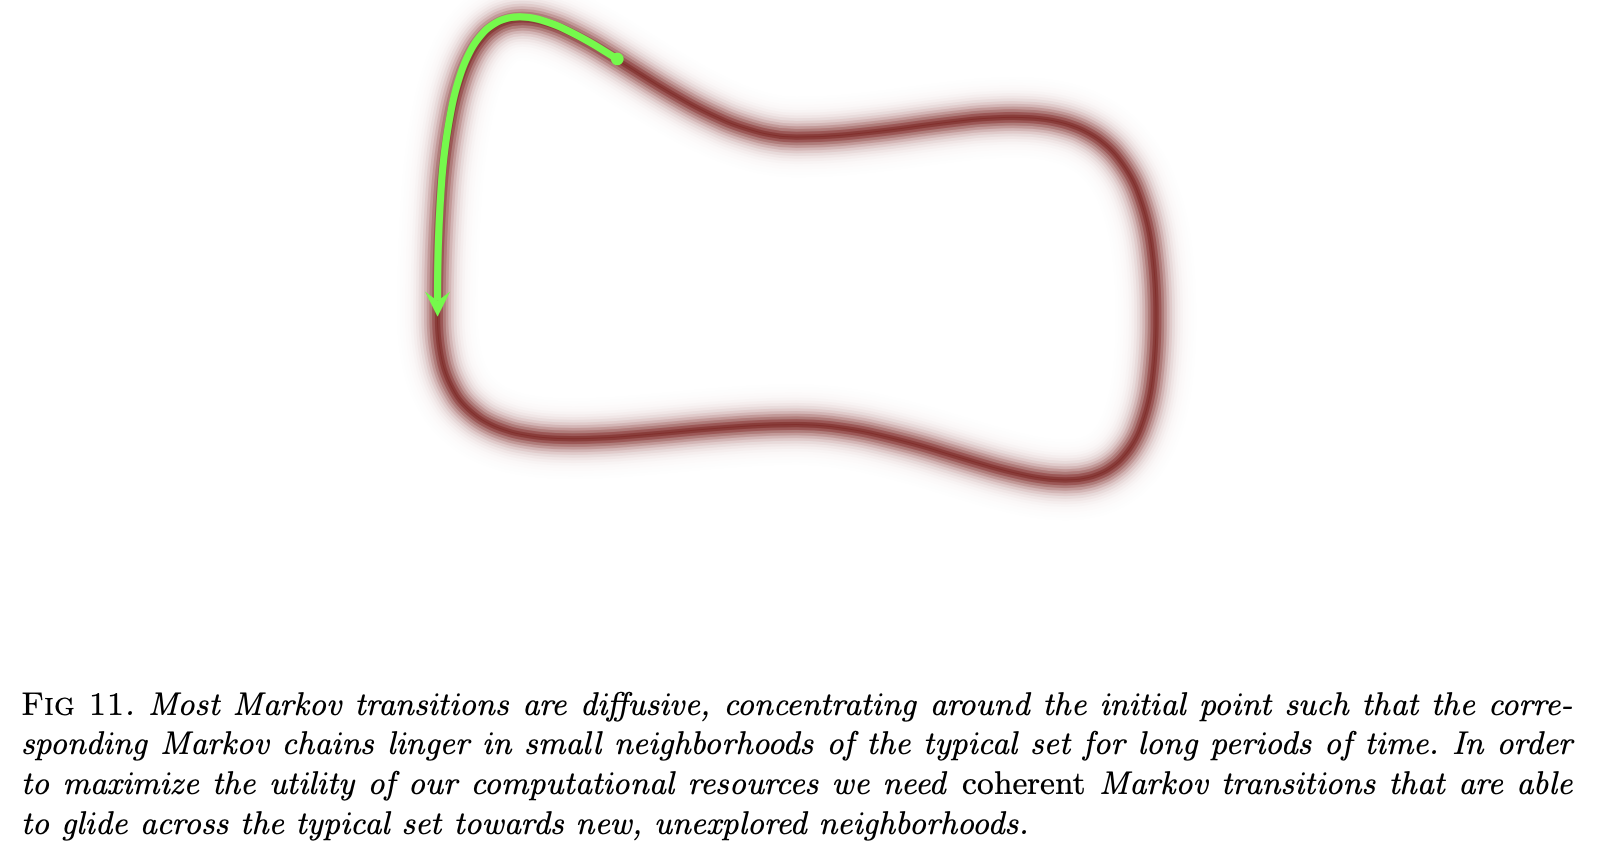
\includegraphics[scale = 0.5]{geometry_explore_typical_set.png}}
\end{minipage}
\caption{\footnotesize{\textbf{The Markov chain that is able to explore the contours of high probability mass is needed.}}}
\label{fig: geometry_explore_typical_set}
\end{figure}

\item In order to make large jumps away from the initial point, and into new, unexplored regions of the typical set, we need to exploit information about the \underline{\textbf{\emph{geometry}}} of the \emph{typical set} itself. Specifically, we need transitions that can follow those \emph{\textbf{contours of high probability mass}}, coherently gliding through the typical set. (Figure \ref{fig: geometry_explore_typical_set})

\item Hamiltonian Monte Carlo is the unique procedure for automatically generating this coherent exploration for sufficiently well-behaved target distributions.
\end{itemize}
\subsection{Hamiltonian Monte Carlo}
\begin{itemize}
\item Compare to MCMC, \underline{\emph{\textbf{Hamiltonian Monte Carlo (HMC)}}} \citep{brooks2011handbook} has some unique characteristics:
\begin{itemize}
\item HMC reply on the \underline{\textbf{\emph{Hamiltonian dynamic}}} to \textbf{explore} the parameter space. As oppose to the \emph{stochastic process} from MCMC, the HMC exploration process is \underline{\emph{\textbf{deterministic}}} based on the \emph{differential equations} \eqref{eqn: Hamilton_equation_1}, \eqref{eqn: Hamilton_equation_2}. HMC only need to simulate the \textbf{initial velocity/momentum} $\mb{v}(0)$ to start the Hamiltonian dynamic.

\item HMC \underline{\textbf{\emph{preserves the target distribution}}} $\pi$ by \emph{properties of Hamiltonian dynamic}, while the MCMC preserve the target distribution as the \emph{stationary distribution} of Markov chain.

\item Unlike the \emph{diffusion transition kernel} in MCMC, the transition process of HMC encodes \underline{\emph{\textbf{geometrical information}}} of the typical set via its associated \emph{\textbf{vector field}}. In other words, instead of fumbling around parameter space with random, uninformed jumps, we can follow the direction assigned to each at point for a small distance.  Continuing this process traces out a coherent trajectory through the typical set that efficiently moves us far away from the initial point to new, unexplored regions of the typical set \emph{as quickly as possible}.  

\item The performance of MCMC and its special case, Gibbs sampling, depend on a particular \emph{\textbf{parameterization}} of the target distribution. On the other hand, the design of Hamiltonian dynamic carefully remove the dependency on parameterization with additional geometric constraints while twisting the directions to align with the typical set. 

\item Compared to Random-walk Metropolis-Hastings, HMC reduces the correlation between successive sampled states by proposing moves to distant states which maintain a high probability of acceptance.
\end{itemize}

\begin{figure}
\begin{minipage}[t]{1\linewidth}
  \centering
  \centerline{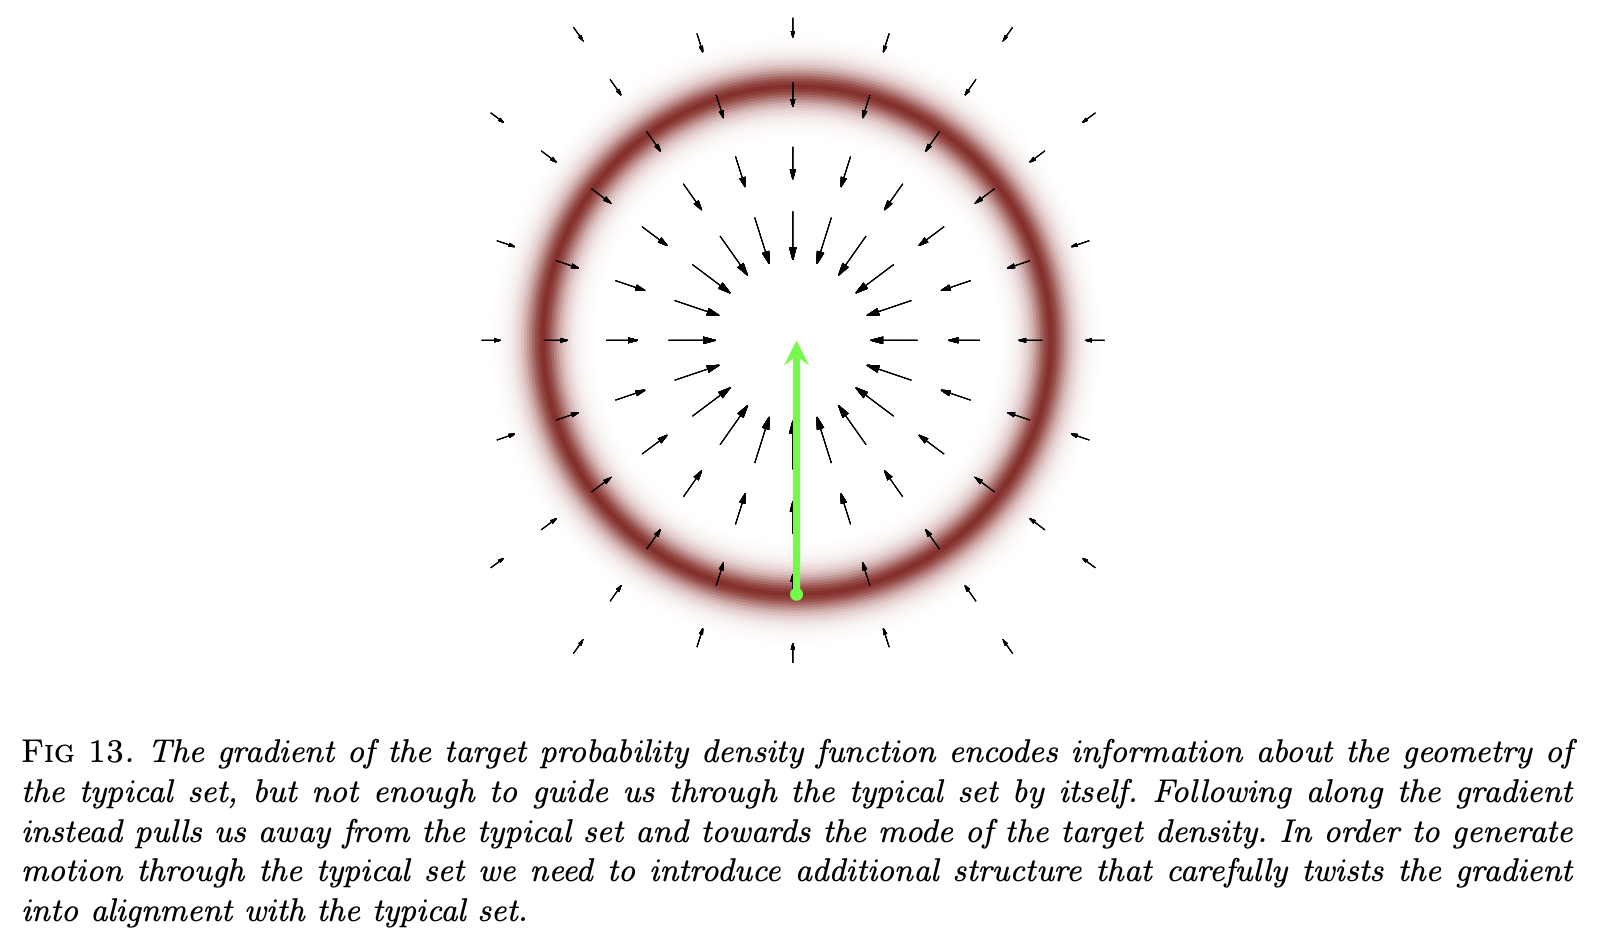
\includegraphics[scale = 0.5]{vector_fields.png}}
\end{minipage}
\caption{\footnotesize{\textbf{The vector fields encode geometrical information and the gradient pull towards the mode of distribution.}}}
\label{fig: vector_fields}
\end{figure}

\item Inspired by classical mechanic systems, the \underline{\textbf{key idea}} of \emph{\textbf{Hamiltonian Monte Carlo (HMC)}} is introduce \emph{\textbf{auxiliary momentum parameters}} in order to twist the gradient vector field into a vector field aligned with the typical set, and hence one capable of generating efficient exploration.

\begin{figure}
\begin{minipage}[t]{1\linewidth}
  \centering
  \centerline{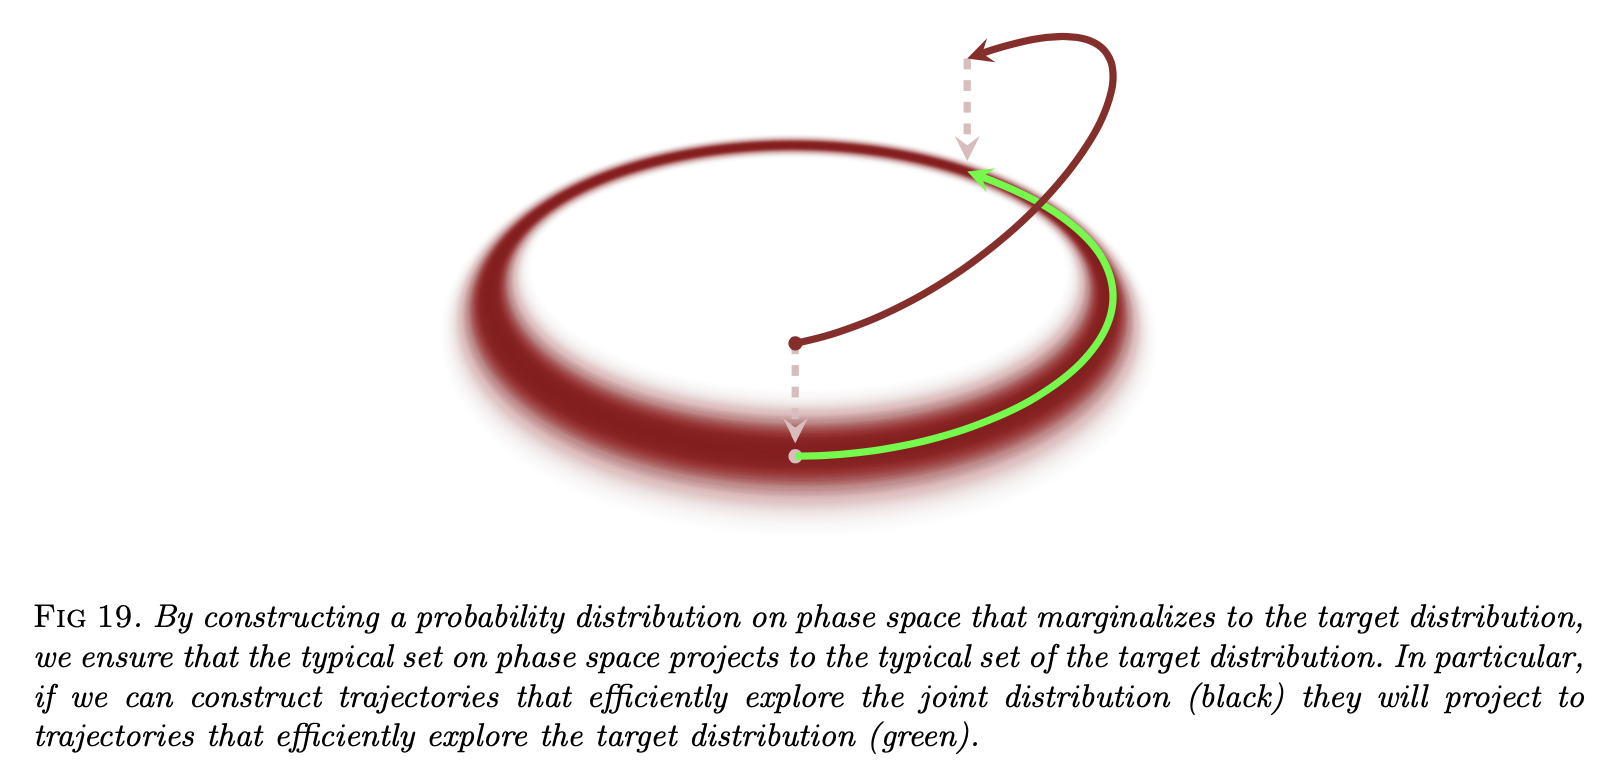
\includegraphics[scale = 0.5]{hmc_circle.png}}
\end{minipage}
\caption{\footnotesize{\textbf{By constructing a probability distribution on phase space that marginalizes to the target distribution, we ensure that the typical set on phase space projects to the typical set of the target distribution. \citep{betancourt2017conceptual}}}}
\label{fig: hmc_circle}
\end{figure}

\item Consider the target distribution as
\begin{align}
\pi(\mb{x}, \mb{v}) &\propto \frac{1}{Z}\exp\paren{-\cH(\mb{x}, \mb{v})}, \label{eqn: hmc_target} 
\end{align} where $\mb{v}$ is the \emph{\textbf{auxiliary momentum parameters}}, $\mb{z} := (\mb{x}, \mb{v})$ is called \emph{\textbf{phase-space parameterization}}. The joint probability $\pi(\mb{x}, \mb{v})$ distribution on phase space is called the \emph{\textbf{canonical distribution}} or phase-space distribution.

Then we can factorize $\pi$ into
\begin{align}
\pi(\mb{x}, \mb{v}) &= \pi(\mb{v}|\mb{x})\pi(\mb{x}) \label{eqn: hmc_factorization} \\
-\log \pi(\mb{x}, \mb{v}) &= -\log \pi(\mb{v}|\mb{x}) - \log \pi(\mb{x}) \nonumber\\
&=\cK(\mb{x}, \mb{v}) + \cV(\mb{x}) := \cH(\mb{x}, \mb{v}).\label{eqn: hmc_factorization_2}
\end{align}  where $\cK(\mb{x}, \mb{v})$ is the \emph{kinetic energy} and $ \cV(\mb{x})$ is the \emph{potential energy}. The potential energy is completely determined by the target distribution while the kinetic energy is \emph{\textbf{unconstrained}} and must be specified by the implementation.

This factorization guarantees that any trajectories exploring the typical set of the phase space distribution $\pi(\mb{x}, \mb{v})$ will project to trajectories exploring the typical set of the target distribution $\pi(\mb{x})$.

\item Note that $\cH(\mb{x}, \mb{v})$ is \underline{\emph{\textbf{independent}}} of the details of any \emph{\textbf{parameterization}}, so does the \emph{canonical density} $\pi(\mb{x}, \mb{v})$ in \eqref{eqn: hmc_target}. Moreover, $\cH(\mb{x}, \mb{v})$ captures the \emph{\textbf{invariant probabilistic structure}} of the phase-space distribution and, most importantly, the \emph{\textbf{geometry}} of its typical set.

\item  Given \eqref{eqn: hmc_factorization_2}, recall from \eqref{eqn: Hamilton_dynamics_general} the Hamilton's equations:
\begin{align}
\frac{d x^{i}}{dt} &=  \partdiff{\cK}{v_{i}} = -\partdiff{\log \pi(\mb{v}|\mb{x})}{v_{i}}, \quad  i=1,\ldots, d \nonumber\\
\frac{d v_{i}}{dt} &= - \partdiff{\cK}{x^{i}} - \partdiff{\cV}{x^{i}} = \partdiff{\log \pi(\mb{v}|\mb{x})}{x^{i}}+\partdiff{\log \pi(\mb{x})}{x^{i}}, \quad  i=1,\ldots, d \label{eqn: hmc_hamiltonian_eqn}
\end{align}

\end{itemize}



\subsection{Idealized Hamiltonian Monte Carlo}
\begin{itemize}
\item Let $\phi_t : (\mb{x}, \mb{v}) \mapsto (\mb{x}_t(\mb{x}, \mb{v}), \mb{v}_t(\mb{x}, \mb{v}))$ be the trajectory characterized by differential equations \eqref{eqn: hmc_hamiltonian_eqn}. $\phi_t(\mb{x}, \mb{v})$ is the position and velocity/momentum at time $t$ starting from $(\mb{x}, \mb{v})$. 

\item The \underline{\emph{\textbf{idealized Hamiltonian Monte Carlo}}} \citep{betancourt2017conceptual, vishnoi2021introduction} is described as below:

\begin{enumerate}
\item For $t=1,2,\ldots, k$:
\begin{enumerate}
\item Given $\mb{X}_{t-1}$, generate a momentum $\mb{V}_{t-1}$ from conditional distribution $\pi(\mb{v}|\mb{X}_{t-1})$;
\item Set $(\mb{X}_{t}, \mb{V}_{t}) = \phi_{T}(\mb{X}_{t-1}, \mb{V}_{t-1})$ by integrating Hamilton’s equations for some time $T$
\end{enumerate}

\item Return $\mb{X}_{k}$ after projecting away the momentum.
\end{enumerate}
Composing these steps together yields a \emph{\textbf{Hamiltonian Markov transition}} composed of \emph{random trajectories} that rapidly explore the target distribution.

\item The sequence $(\mb{X}_{t}, \mb{V}_{t})$ is a \textbf{Markov chain} since $(\mb{X}_{t+1}, \mb{V}_{t+1})$ only depends on the initial condition of Hamiltonian dynamic $(\mb{X}_{t}, \mb{V}_{t})$. Consequently, the sub-chain $(\mb{X}_{t})$ is also a Markov chain.

\item Note that since the Hamiltonian dynamic remains in typical set throughout iterations, there is no need for rejection, i.e. the acceptance rate is $1$. Given $T$ large enough, a new sample $\mb{X}_{t+1}$ would have less correlation to $\mb{X}_{t}$. Thus it is expected that 
\end{itemize}

\subsection{The Natural Geometry of Phase Space}
\begin{itemize}
\item One of the characteristic properties of Hamilton’s equations is that they \emph{conserve the value of the Hamiltonian}. In other words, every Hamiltonian trajectory is confined to an \emph{\textbf{energy level set}},
\begin{align*}
\cH^{-1}(E) &= \set{(\mb{x}, \mb{v}): \cH(\mb{x}, \mb{v}) = E},
\end{align*} which, save for some ignorable exceptions, are all $(2\,d - 1)$-dimensional, \emph{\textbf{compact}} surfaces in phase space. In fact, once we’ve removed any singular level sets, the entirety of phase space neatly decomposes, or \emph{\textbf{foliates}} into \emph{\textbf{concentric level sets}}. Consequently, we can specify any point in phase space by first specifying the energy of the level set it falls on, $E$, and the position within that level set, $\mb{\theta}_{E}$. 

\item Correspondingly the canonical distribution on phase space admits a \emph{\textbf{microcanonical decomposition}},
\begin{align*}
\pi(\mb{x}, \mb{v}) &= \pi(\mb{\theta}_{E}\,|\,E)\pi(E),
\end{align*} across this \emph{\textbf{foliation}}. The conditional distribution over each level set, $\pi(\mb{\theta}_{E}\,|\,E)$, is called the \emph{\textbf{microcanonical distribution}}, while the distribution across the level sets, $\pi(E)$, is called the \emph{\textbf{marginal energy distribution}}.

\begin{figure}
\begin{minipage}[t]{1\linewidth}
  \centering
  \centerline{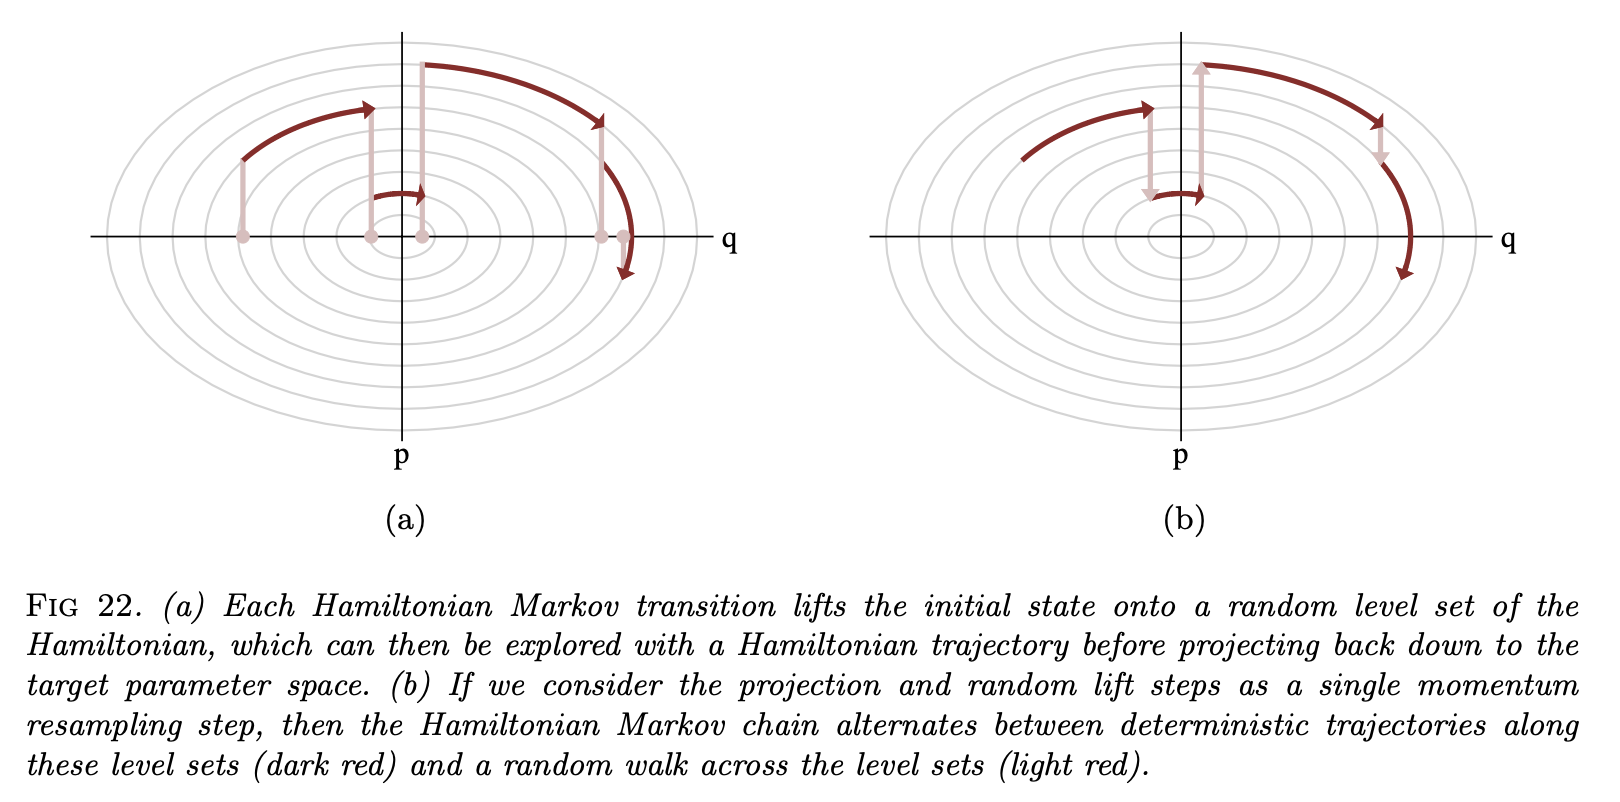
\includegraphics[scale = 0.5]{hmc_geomotry_process.png}}
\end{minipage}
\caption{\footnotesize{\textbf{Using level-sets, we see that HMC first explore within level set and then jump from one level set to another via random walk. \citep{betancourt2017conceptual}}}}
\label{fig: hmc_geomotry_process}
\end{figure}

\item This microcanonical decomposition is particularly well-suited to analyzing the Hamiltonian transition. To see this more clearly, consider a Hamiltonian Markov chain consisting of multiple transitions. Each Hamiltonian trajectory explores a level set while the intermediate \emph{projections} and \emph{lifts} define a random jump between the level sets themselves. Consequently, the entire Hamiltonian Markov chain decouples into \textbf{\emph{two distinct phases}}: 
\begin{enumerate}
\item \emph{\textbf{deterministic}} exploration of individual \emph{level sets}
\item a \emph{\textbf{stochastic}} exploration \emph{\textbf{between}} the level sets themselves 
\end{enumerate}
\end{itemize}


\subsection{Property of Hamiltonian Monte Carlo}
\begin{itemize}
\item Let $\mu$ be the Lebesgue measure on $\bR^d \times \bR^d$ with respect to which all densities are defined.
\begin{theorem} (HMC Preserves the Target Density) \citep{vishnoi2021introduction}
Suppose $(\mb{X}, \mb{V})$ is a sample from the density
\begin{align*}
\pi(\mb{x}, \mb{v}) &= \frac{1}{Z}\exp\paren{-\cH(\mb{x}, \mb{v})}d\mu(\mb{x}, \mb{v})
\end{align*} where $Z = \int \exp\paren{-\cH(\mb{x}, \mb{v})}d\mu(\mb{x}, \mb{v})$ is the partition function. Let $T > 0$ be the step size of the HMC. Then the density of $\phi_T(\mb{X}, \mb{V})$ is $\pi$ for any $T \ge 0$. Moreover the density of $\phi_T(\mb{X}_{t-1}, \mb{V}_{t-1})$, where $\mb{V}_{t-1} \sim \pi(\mb{v}|\mb{X}_{t-1})$ is also $\pi$. Thus, the idealized HMC algorithms preserves $\pi$.
\end{theorem}
\begin{proof}
For $T \ge 0$, let $(\widehat{\mb{x}}, \widehat{\mb{v}}) = \phi_T(\mb{x}, \mb{v})$. Then, it follows from the \emph{preservation of Hamiltonian along trajectories} that
\begin{align*}
\cH(\widehat{\mb{x}}, \widehat{\mb{v}}) = \cH(\phi_T(\mb{x}, \mb{v}))  &= \cH(\mb{x}, \mb{v}).
\end{align*}
Thus the function $\exp(-\cH(\mb{x}, \mb{v})) = \exp(-\cH(\widehat{\mb{x}}, \widehat{\mb{v}}))$

Let $\mu^{*}$ be the \emph{pushforward} of $\mu$ under the map $\phi_{T}$, i.e. $(\phi_{T})_{\#}\mu = \mu^{*}$. The property that Hamiltonian dynamics \emph{preserves volume} in phase space states that the determinant of the Jacobian of the map $\phi_{T}$, $\det\paren{\partial_{\mb{z}}\mb{\phi}_T} = 1$.
Therefore, 
\begin{align*}
 d\mu^{*} &= \det\paren{\partial_{\mb{z}}\mb{\phi}_T}\,d\mu= d\mu, 
\end{align*} i.e. $\mu^{*} = \mu$. Thus, the normalization factor
\begin{align*}
Z^{*}=  \int \exp(-\cH(\widehat{\mb{x}}, \widehat{\mb{v}}))d\mu^{*} &=  \int \exp(-\cH(\mb{x}, \mb{v}))d\mu = Z.
\end{align*} Therefore the target distribution $\pi$ remains invariant under $\phi_{T}$. \qed
\end{proof}
\end{itemize}

\subsection{Euclidean-Gaussian Kinetic Energies}
\begin{itemize}
\item The first substantial \textbf{\emph{degree of freedom}} in the Hamiltonian Monte Carlo method that we can tune is the choice of the conditional probability distribution over the momentum or, equivalently, \textbf{the choice of a kinetic energy function}. Along with the target distribution, this choice completes the probabilistic structure on phase space which then determines the geometry of the microcanonical decomposition.

\item The simplest choice is to allow velocity/momentum $\mb{V}_{t}$ being \textbf{\emph{independent}} of $\mb{X}_{t}$, i.e. $\pi(\mb{v}|\mb{x}):= g(\mb{v})$. This is equivalent to assuming that \emph{the phase-space geometry} is \emph{\textbf{flat}}. The Hamiltonian Monte Carlo corresponds to a \emph{random-walk} across a foliation of the phase-space.

\item A natural choice of $g(\mb{v})$ is Normal distribution $\cN(\mb{v}\,|\, \mb{0}, \mb{\Sigma}_{v})$. Here, the covariance matrix $\mb{\Sigma}_{v}$ encodes an Euclidean metric in the phase-space. The corresponding kinetic energy is a \emph{\textbf{Euclidean-Gaussian kinetic energy}}
\begin{align}
\cK(\mb{v}) &= \frac{1}{2}\mb{v}^{T} \mb{\Sigma}_{v}^{-1} \mb{v} + \log \det{\mb{\Sigma}_{v}} + const.. \label{eqn: hmc_quatratic_kinetic}
\end{align}   And the Hamilton's equation is simplified as 
\begin{align}
\frac{d \mb{x}}{dt} &= \grad{\mb{v}}{\cK} = \mb{\Sigma}_{v}^{-1} \mb{v}  \nonumber\\
\frac{d \mb{v}}{dt} &= - \grad{\mb{x}}{\cV} = \grad{\mb{x}}{E} \label{eqn: hmc_hamiltonian_eqn_quar_k}
\end{align} where the target distribution $\pi(\mb{x}) \propto \exp(-E(\mb{x}))$.

In the physical perspective the Euclidean metric $\mb{\Sigma}_{v}$ is known as the \emph{\textbf{mass matrix}}, a term that has consequently become common in the Hamiltonian Monte Carlo literature.

\item Because the Euclidean structure over the momentum is dual to the Euclidean structure over the parameters, its interactions with the target distribution are straightforward to derive. Applying the transformation $\mb{p}' = \mb{\Sigma}_v^{-1/2}\mb{v}$ simplifies the kinetic energy, but remember that we have to apply the \emph{\textbf{opposite transformation}} to the parameters, $\mb{x}' = \mb{\Sigma}_v^{1/2}\mb{x}$, to preserve the Hamiltonian geometry.  Consequently, a choice of $\mb{\Sigma}_{v}^{-1}$ effectively \emph{\textbf{rotates}} and then \emph{\textbf{rescales}} the target \textbf{parameter} space, potentially \emph{\textbf{correlating}} or \textbf{\emph{de-correlating}} the target distribution and correspondingly \emph{\textbf{warping}} the energy level sets.

In particular, as the inverse Euclidean metric more closely resembles the covariance of the target distribution it de-correlates the target distribution, resulting in energy level sets that are more and more uniform and hence easier to explore. 

\item Thus the \emph{\textbf{optimal choice}} of Euclidean-Gaussian kinetic energy is the \emph{inverse} of covariance on $\mb{x}$:
\begin{align*}
\mb{\Sigma}_{v}^{-1} &= \E{\pi}{\paren{\mb{X}-\mb{\mu}_{X}}\paren{\mb{X}-\mb{\mu}_{X}}^{T}}
\end{align*}


\end{itemize}


\section{Hamiltonian Monte Carlo in Practice}
\begin{itemize}
\item The \underline{\emph{\textbf{main obstruction}}} to implementing the Hamiltonian Monte Carlo method is \textbf{generating} the Hamiltonian \textbf{trajectories} themselves. Aside from a few trivial examples, we \emph{cannot solve Hamilton’s equations exactly} and any implementation must instead solve them numerically. \textbf{Numerical inaccuracies}, however, can quickly compromise the utility of even the most well-tuned Hamiltonian transition. 

\begin{figure}
\begin{minipage}[t]{1\linewidth}
  \centering
  \centerline{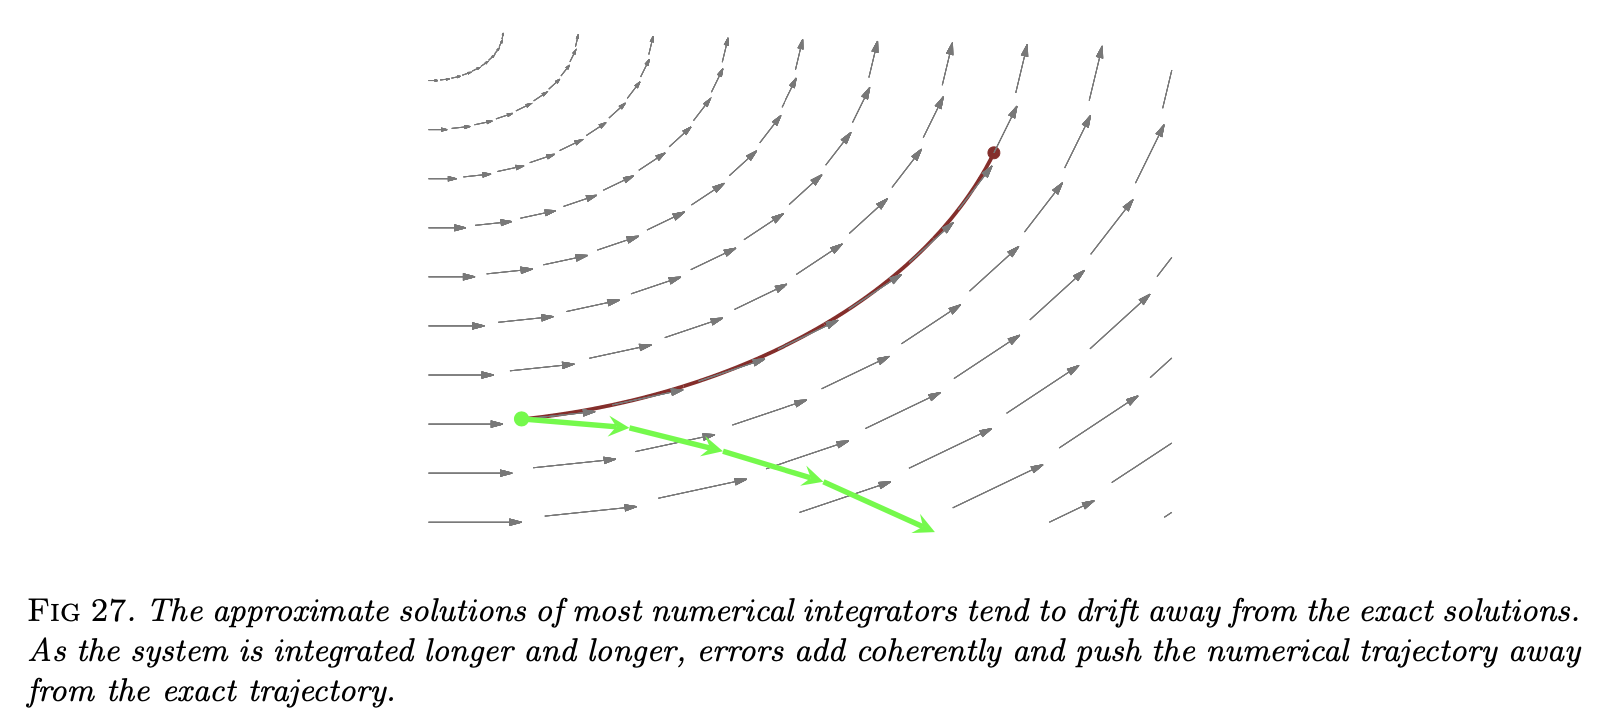
\includegraphics[scale = 0.5]{hmc_trajectory_sim_fail.png}}
\end{minipage}
\caption{\footnotesize{\textbf{Most numerical methods for PDE does not preserve volume. \citep{betancourt2017conceptual}}}}
\label{fig: hmc_trajectory_sim_fail}
\end{figure}

The more accurately we can numerically solve the system of ODEs, the more effective our implementation will be.

\item Common ODE solvers suffer from an issue of \emph{\textbf{drift}}. As we numerically solve longer and longer trajectories the error in the solvers adds coherently, pushing the approximate trajectory away from the true trajectory and the typical set that we want to explore (Figure \ref{fig: hmc_trajectory_sim_fail}). Moreover, the magnitude of this drift rapidly increases with the dimension of phase space. Thus these solvers are limited to solve short Hamiltonian trajectories, which is inefficiently explore the energy level sets.

\item Fortunately, we can use the geometry of phase space itself to construct an extremely powerful family of numerical solvers, known as \underline{\emph{\textbf{symplectic integrators}}} \citep{liu2001monte, leimkuhler2004simulating, haier2006geometric, betancourt2017conceptual, vishnoi2021introduction}, that are robust to phenomena like drift and enable high-performance implementations of the Hamiltonian Monte Carlo method.
\end{itemize}

\subsection{Symplectic Integrators}
\begin{itemize}
\item Symplectic integrators are powerful because the numerical trajectories they generate exactly \emph{\textbf{preserve phase space volume}}, just like the Hamiltonian trajectories they are approximating. Consequently, the numerical trajectories cannot drift away from the exact energy level set, instead oscillating near it even for long integration times.

\begin{figure}
\begin{minipage}[t]{1\linewidth}
  \centering
  \centerline{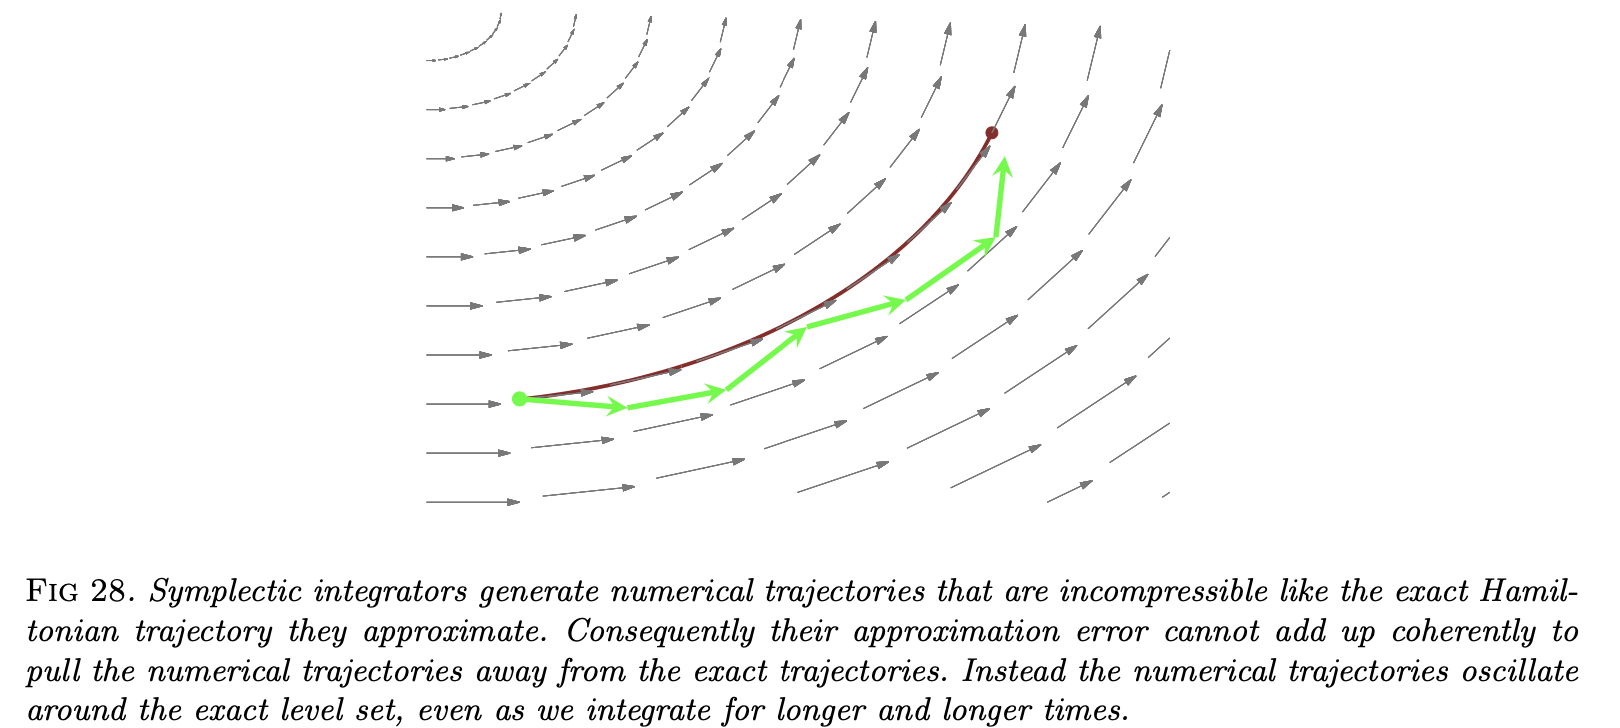
\includegraphics[scale = 0.5]{symplectic_integrator.png}}
\end{minipage}
\caption{\footnotesize{\textbf{Symplectic integrator will oscillate near exact level set even for long integration times. \citep{betancourt2017conceptual}}}}
\label{fig: symplectic_integrator}
\end{figure}


\item For independent momentum distribution like the Euclidean-Gaussian kinetic energy, the symplectic integrator is called \emph{\textbf{leapfrog integrator}} \citep{brooks2011handbook}. 

\item The \underline{\emph{\textbf{Leapfrog Integrator}}} is described as below, where  $\epsilon$ is the time discretization, or step size:
\begin{enumerate}
\item Initialization: $\mb{x}_0 \leftarrow \mb{x}$, $\mb{v}_0 \leftarrow \mb{v}$.
\item For $0 \le t \le \lfloor \frac{T}{\epsilon}\rfloor$:
\begin{flalign*}
(a)\quad &\mb{v}_{t+\frac{1}{2}} \leftarrow \mb{v}_{t} - \frac{\epsilon}{2}\grad{\mb{x}}{\cV}(\mb{x}_{t})&\\
(b)\quad &\mb{x}_{t+1} \leftarrow \mb{x}_{t} + \epsilon\, \mb{\Sigma}_{v}^{-1}\mb{v}_{t+\frac{1}{2}}\\
(c)\quad &\mb{v}_{t+1} \leftarrow \mb{v}_{t+\frac{1}{2}} - \frac{\epsilon}{2}\grad{\mb{x}}{\cV}(\mb{x}_{t+1})
\end{flalign*}
\end{enumerate}

This simple but precise interleaving of discrete momentum and position updates ensures exact volume preservation on phase space, and hence the accurate numerical trajectories we need to realize the potential of a Hamiltonian transition.


\item Employing symplectic integrators provides the opportunity to translate the theoretical performance of the Hamiltonian Monte Carlo method into a practical implementation. There remain, however, two obstructions to realizing this translation. 
\begin{itemize}
\item First, even though symplectic integrators are highly accurate, the small errors they do introduce will bias the resulting Hamiltonian transitions without an exact correction. 
\item Second, we have to be able to select a symplectic integrator well-suited to a given target distribution.
\end{itemize}

\begin{figure}
\begin{minipage}[t]{1\linewidth}
  \centering
  \centerline{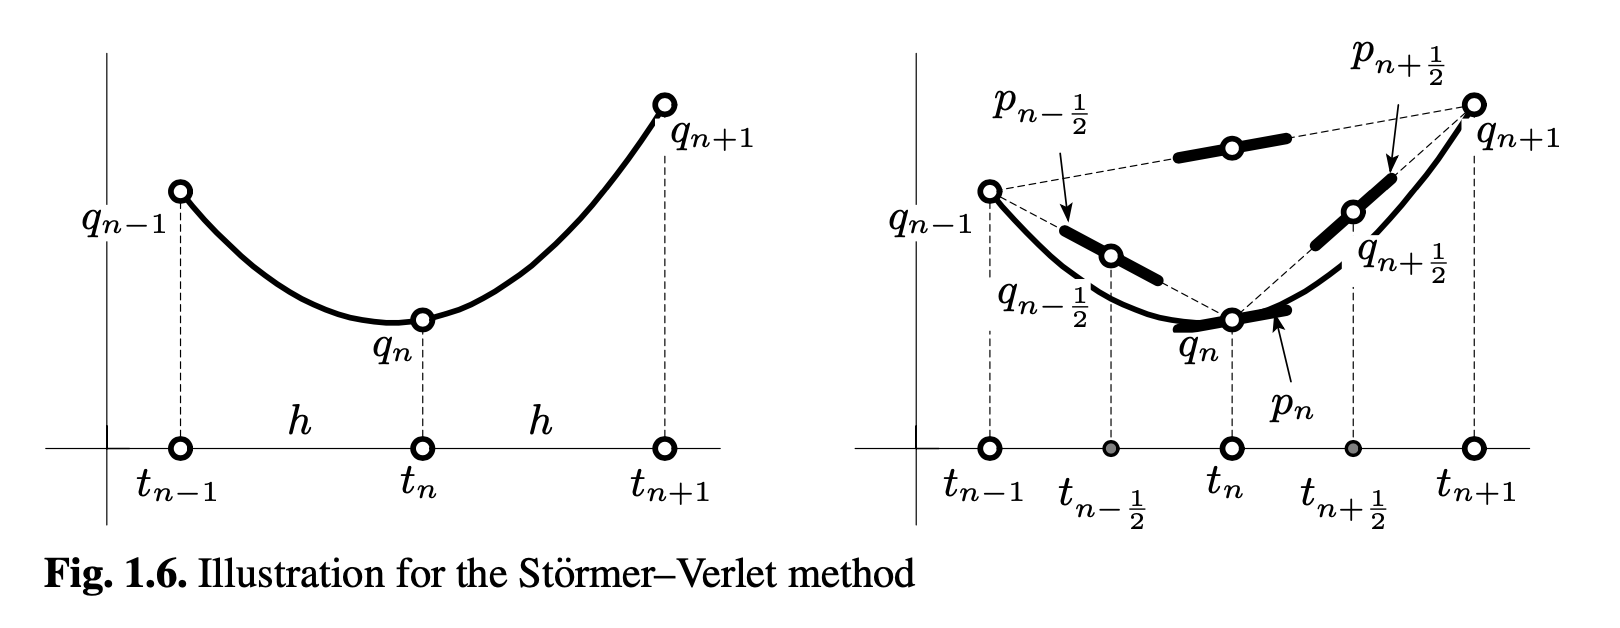
\includegraphics[scale = 0.5]{leapfrog.png}}
\end{minipage}
\caption{\footnotesize{\textbf{Leapfrog integrator can be seen as produced by parabolas \citep{haier2006geometric}}}}
\label{fig: leapfrog}
\end{figure}


\end{itemize}

\subsection{Correcting for Symplectic Integrator Error}
\begin{itemize}
\item One particularly natural strategy for correcting the bias introduced by the error in a symplectic integrator is to treat the \emph{\textbf{Hamiltonian transition as the proposal}} for a Metropolis-Hastings scheme on phase space. 

\item Suppose $(\mb{x}_{L}, \mb{v}_{L})$ be the last state of $L$ symplectic integrator steps starting from $(\mb{x}_{0}, \mb{v}_{0})$. We are interested in the \emph{Hastings ratio} (i.e. the acceptance rate threshold):
\begin{align*}
r(\mb{x}_{0}, \mb{v}_{0}; \mb{x}_{L}, \mb{v}_{L}) &=\frac{\pi(\mb{x}_{L}, \mb{v}_{L})\,K((\mb{x}_{L}, \mb{v}_{L}); (\mb{x}_{0}, \mb{v}_{0}))}{\pi(\mb{x}_{0}, \mb{v}_{0})\,K((\mb{x}_{0}, \mb{v}_{0}); (\mb{x}_{L}, \mb{v}_{L}))} 
\end{align*} where $K((\mb{x}_{0}, \mb{v}_{0}); (\mb{x}_{L}, \mb{v}_{L})):= T\set{(\mb{x}_{0}, \mb{v}_{0})\rightarrow (\mb{x}_{L}, \mb{v}_{L})} = \delta_{\mb{x}_{0}}(\mb{x}_{L})\,\delta_{\mb{v}_{0}}(\mb{v}_{L})$ is the transition kernel (rule) from $(\mb{x}_{0}, \mb{v}_{0})$ to  $(\mb{x}_{L}, \mb{v}_{L})$. For HMC, this transition is achieved via numerical integrator simulating the Hamilton dynamics. 

For a given integrator, because we can propose only states going forwards and not backwards, this ratio is always $0$.

\item If we modify the Hamiltonian transition to be \emph{\textbf{reversible}}, however, then the ratio of proposal densities becomes non-zero and we achieve a useful correction scheme. The simplest way of achieving a reversible proposal is to augment the the numerical integration with a negation step that \underline{\emph{\textbf{flips the sign of momentum}}}. Thus the reverse proposal is 
\begin{align*}
K((\mb{x}_{L}, -\mb{v}_{L}); (\mb{x}_{0}, \mb{v}_{0})) &:= T\set{(\mb{x}_{L}, -\mb{v}_{L})\rightarrow (\mb{x}_{0}, \mb{v}_{0})}\\
&= \delta_{\mb{x}_{L}}(\mb{x}_{0})\,\delta_{-\mb{v}_{L}}(\mb{v}_{0})
\end{align*}


\begin{figure}
\begin{minipage}[t]{1\linewidth}
  \centering
  \centerline{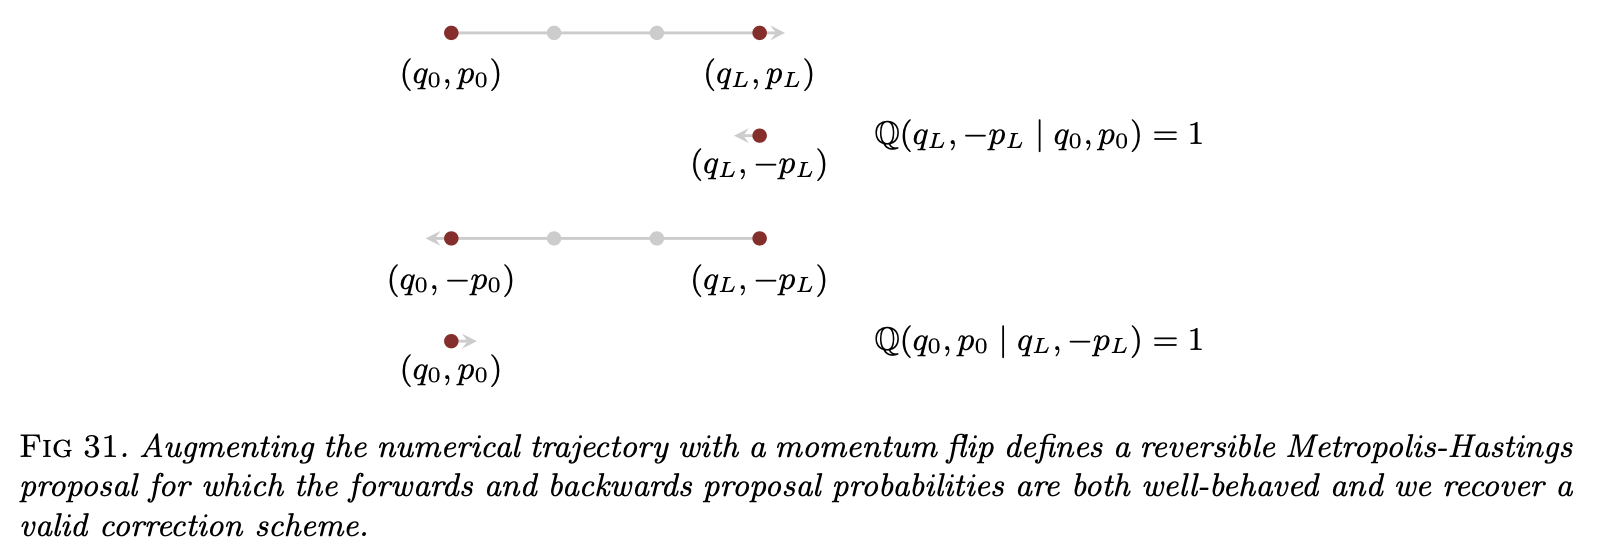
\includegraphics[scale = 0.6]{metro_hmc.png}}
\end{minipage}
\caption{\footnotesize{\textbf{Obtaining the reverse chain by flipping the sign of momentum. Note that the kinetic energy is symmetric to the change of sign in momentum. \citep{betancourt2017conceptual}}}}
\label{fig: metro_hmc}
\end{figure}

\item The \emph{\textbf{Hastings ratio}} is then computed as
\begin{align}
r(\mb{x}_{0}, \mb{v}_{0}; \mb{x}_{L}, -\mb{v}_{L}) &=\frac{\pi(\mb{x}_{L}, -\mb{v}_{L})\,K((\mb{x}_{L}, -\mb{v}_{L}); (\mb{x}_{0}, \mb{v}_{0}))}{\pi(\mb{x}_{0}, \mb{v}_{0})K((\mb{x}_{0}, \mb{v}_{0}); (\mb{x}_{L}, -\mb{v}_{L}))}  \nonumber\\
&= \frac{\pi(\mb{x}_{L}, -\mb{v}_{L})\,\delta_{\mb{x}_{L}}(\mb{x}_{0})\,\delta_{-\mb{v}_{L}}(\mb{v}_{0})}{\pi(\mb{x}_{0}, \mb{v}_{0})\,\delta_{\mb{x}_{0}}(\mb{x}_{L})\,\delta_{\mb{v}_{0}}(-\mb{v}_{L})}\nonumber\\
&=  \frac{\pi(\mb{x}_{L}, -\mb{v}_{L})}{\pi(\mb{x}_{0}, \mb{v}_{0})} = \frac{\exp(-\cH(\mb{x}_{L}, -\mb{v}_{L}))}{\exp(-\cH(\mb{x}_{0}, \mb{v}_{0}))} \nonumber\\
&= \exp\paren{-\cH(\mb{x}_{L}, -\mb{v}_{L}) + \cH(\mb{x}_{0}, \mb{v}_{0})}\label{eqn: hmc_hastings_ratio}
\end{align}

\item Finally, we have \underline{\emph{\textbf{Metropolized Hamiltonian Monte Carlo}}} \citep{brooks2011handbook, betancourt2017conceptual}:
\begin{enumerate}
\item For $t=1,2,\ldots, k$:
\begin{enumerate}
\item Generate a momentum $\mb{V}_{t-1}$ from Normal distribution $\cN(\mb{0}, \mb{\Sigma}_{v})$;
\item Set $(\mb{X}', \mb{V}') = \widehat{\phi}_{T}(\mb{X}_{t-1}, \mb{V}_{t-1})$ as the last state of $T$ symplectic integrator steps starting from 
$(\mb{X}_{t-1}, \mb{V}_{t-1})$. 

\item Compute the Hastings ratio:
\begin{align*}
r(\mb{X}_{t-1}, \mb{V}_{t-1}; \mb{X}', -\mb{V}') &= \exp\paren{-\cH(\mb{X}', -\mb{V}') + \cH(\mb{X}_{t-1}, \mb{V}_{t-1})}
\end{align*}

\item Accept $\mb{X}_{t} = \mb{X}'$ with probability 
\begin{align*}
\alpha(\mb{X}_{t-1}, \mb{V}_{t-1}; \mb{X}', -\mb{V}') &= \min\set{1,\;r(\mb{X}_{t-1}, \mb{V}_{t-1}; \mb{X}', -\mb{V}')}
\end{align*}

\item Otherwise, accept $\mb{X}_{t} = \mb{X}_{t-1}$.
\end{enumerate}
\end{enumerate}

\item Symplectic integrators are not exactly energy preserving, causing their numerical trajectories to deviate from the target energy level set. In particular, sampling a state uniformly from any numerical trajectory will not generate a sample from the canonical distribution. This error, however, can be exactly corrected by sampling from the trajectory not uniformly but rather with weights proportional to the desired canonical density function \citep{betancourt2017conceptual}.

\item Regarding the \emph{\textbf{robustness}} of the HMC, preliminary results show that even simple implementations of the Hamiltonian Monte Carlo method are geometrically ergodic over a large class of target distributions, larger than the class for non-gradient based algorithms like Random-walk Metropolis-Hastings.

\item There also some concerns in practice:
\begin{itemize}
\item In practice, \emph{\textbf{longer trajectory}} $T$ is preferred so that the end state is less correlated with the initial state. However, it will have larger cost of simulation time.

\item Also, if the \emph{\textbf{kinetic energy}} is \emph{poorly-chosen} then the marginal energy distribution can become heavy-tailed itself in which case the stochastic exploration between level sets will become so slow that after any finite number of transitions the exploration of the Markov chain will be incomplete.

\item Another common obstruction to geometric ergodicity is neighborhoods in parameter space where the target distribution exhibits \emph{\textbf{large curvature}}. Most Markov transitions are not able to resolve these narrow neighborhoods, resulting in incomplete exploration and biased Markov chain Monte Carlo estimators. 

\item Finally, HMC requires computation on the \emph{\textbf{gradients}} in the symplectic integrator. It would be computational expensive if the target distribution has complex form.
\end{itemize}
\end{itemize}



\section{Connections with Information Geometry}
\begin{itemize}
\item It can be established that the performance of HMC depends on the geometrical property of the target distributions. 

\item \begin{theorem} \citep{vishnoi2021introduction}\\
Let $\cV: \bR^d \rightarrow \bR$  be a twice-differentiable function which satisfies $m\,\mb{I}_{d} \preceq \nabla^2_{\mb{x}}\paren{\cV(\mb{x})} \preceq M\,\mb{I}_{d}$. Let $\mu_k$ be the distribution of $\mb{X}_{k}$ at step $k$ from \textbf{the Idealized HMC}. Suppose that both $\mu_{0}$
and $\pi$ have mean and variance bounded by $\cO(1)$. Then given any $\epsilon > 0$, for $T = \Omega(\frac{\sqrt{m}}{M})$ and $k = \cO((M/m)^2\, \log(1/\epsilon))$, we have that $\cW_{2}(\mu_{k},\pi) \le \epsilon$. 
\end{theorem}
\end{itemize}



\newpage
\bibliographystyle{plainnat}
\bibliography{book_reference.bib}
\end{document}